%!TEX root = thesis.tex


\chapter{SWEET-Cat}
\label{sec:SWEET-Cat}

Part of the work during the thesis has been dedicated to regularly update
SWEET-Cat\footnote{\url{https://www.astro.up.pt/resources/sweet-cat/}}, a catalogue with all
discovered planet hosts, and the stellar parameters.

In this chapter a detailed description of SWEET-Cat will be presented. Moreover an analysis of 50
planet hosts was performed during the thesis with updated planetary parameters (mass and radius).


\section{What is SWEET-Cat?}

As mentioned above, SWEET-Cat is a catalogue of planet host stars. However, the strength of
SWEET-Cat is the homogeneously analysed stars utilising the method described in
\sref{sec:parameters} with \code{FASMA} or a similar tool before the creation of \code{FASMA}.

In the era with a large number of discovered exoplanets (more than 3500 confirmed exoplanet at the
moment of writing), the time for in-depth statistical studies has arrived. However, when conducting
these studies it is crucial to have consistent measurements of e.g. stellar atmospheric parameters.
This can be obtained by using a single analysis to obtain these parameters, as it is know that
different methods will lead to different results \citep[see e.g.][for a recent review]{Hinkel2016}.

To obtain stellar atmospheric parameters from one method is an on-going goal with SWEET-Cat, where
high quality spectra are obtained for stars hosting planets. These are used to determine the stellar
parameters in a homogeneous way. All stars in SWEET-Cat analysed with the method from our group are
marked with a flag showing whether it is analysed homogeneously or not. The columns provided in
SWEET-Cat are summarised in \tref{tab:sweetcat}. It is important to note that SWEET-Cat does not
include any planetary parameters.

\begin{table}[htb!]
    \caption{Columns in SWEET-Cat}
    \label{tab:sweetcat}
    \centering
    \begin{tabular}{lrl}
      \hline\hline
      Column                         & Unit      & Description \\
      \hline
      Name                           &           & Popular stellar name                                 \\
      HD number                      &           & HD number                                            \\
      RA                             & \si{deg}  & Right ascension                                      \\
      Dec                            & \si{deg}  & Declination                                          \\
      $\mathrm{Vmag}$                & \si{mag}  & V magnitude                                          \\
      $\sigma(\mathrm{Vmag})$        & \si{mag}  & Error on V magnitude                                 \\
      $\pi$                          & \si{mas}  & Parallax                                             \\
      $\sigma(\pi)$                  & \si{mas}  & Error on parallax                                    \\
      Source of $\pi$                &           & Source of parallax measurement                       \\
      $T_\mathrm{eff}$               & \si{K}    & Effective temperature                                \\
      $\sigma(T_\mathrm{eff})$       & \si{K}    & Error on effective temperature                       \\
      $\log g$                       & \si{dex}  & Surface gravity                                      \\
      $\sigma(\log g)$               & \si{dex}  & Error on surface gravity                             \\
      $\log g_{\mathrm{LC}}$         & \si{dex}  & Surface gravity corrected from light curves          \\
      $\sigma(\log g_{\mathrm{LC}})$ & \si{dex}  & Error on surface gravity corrected from light curves \\
      $\xi_\mathrm{micro}$           & \si{km/s} & Micro turbulence                                     \\
      $\sigma(\xi_\mathrm{micro})$   & \si{km/s} & Error on micro turbulence                            \\
      $[\ion{Fe}/\ion{H}]$           & \si{dex}  & Metallicity                                          \\
      $\sigma([\ion{Fe}/\ion{H}])$   & \si{dex}  & Error on metallicity                                 \\
      Mass                           & $M_\odot$ & Stellar mass                                         \\
      $\sigma(\mathrm{Mass})$        & $M_\odot$ & Error on stellar mass                                \\
      Reference                      &           & Reference for parameters                             \\
      Homogeneity flag               & 0/1       & 0 for not homogeneous analysis, 1 otherwise          \\
      Last updated                   & date      & Last updated                                         \\
      Comments                       &           & Any special remarks/comments (e.g. M star)           \\
      \hline
    \end{tabular}
\end{table}

SWEET-Cat is updated on a weekly basis if new planet hosts are discovered, and whenever planet hosts
have been analysed with the method from our group, as described in this thesis.


\section{Data for 50 planet hosts}

In this section the data for a large update to SWEET-Cat will be described. The majority of the data
comes as a result from proposals submitted for observational time, while some of the data was found
in the archive. In the next section the analysis of the 50 spectra will be presented along with the
results.



\subsection{Data collected from proposals}

Data\footnote{Based on observations collected at the La Silla Observatory, ESO (Chile), with
FEROS/2.2m (run 2014B/020), with UVES/VLT at the Cerro Paranal Observatory (runs ID 092.C-0695,
093.C-0219, 094.C-0367, 095.C-0324, and 096.C-0092), and with FIES/NOT at Roque de los Muchachos
(Spain) (runs ID 14AF14 and 53-202).} for 43 out of the 50 stars were collected by the SWEET-Cat
team using the UVES/VLT \citep{UVES}, FEROS/2.2m telescope in La Silla \citep{FEROS}, and FIES/NOT
\citep{FIES} spectrographs. The remaining spectra were found in various archives. This includes
spectra from the HARPS/3.6m telescope in La Silla \citep{HARPS} and ESPaDOnS/CFHT \citep{ESPADONS}.
Some characteristics of the spectrographs are presented in \tref{tab:instruments} with the mean S/N
for the spectra used. The S/N for each star can be seen in \tref{tab:SCresults} along with the
atmospheric parameters of the stars. The S/N is measured automatically by ARES, however note that
ARES smoothes the spectra before measuring the S/N, hence it is listed higher than the actual S/N.
These 50 stars are confirmed exoplanet hosts listed in SWEET-Cat, but they belonged to the list of
stars that have not previously been analysed by our team.


\begin{table}[htb!]
    \caption{Spectrographs used for this paper with their spectral resolution,
             wavelength coverage, and mean S/N from the spectra used.}
    \label{tab:instruments}
    \centering
    \begin{tabular}{llll}
      \hline\hline
      Spectrograph & Resolution    & Spectral range            &   Mean S/N  \\
      \hline
      HARPS        &  \num{115000} & \SIrange{378}{691}{nm}    &   642       \\
      UVES         &  \num{110000} & \SIrange{480}{1100}{nm}   &   212       \\
      ESPaDOnS     &   \num{81000} & \SIrange{370}{1050}{nm}   &   775       \\
      FIES         &   \num{67000} & \SIrange{370}{730}{nm}    &   763       \\
      FEROS        &   \num{48000} & \SIrange{350}{920}{nm}    &   208       \\
      \hline
    \end{tabular}
\end{table}


\subsection{Data collected from archive}

The spectra\footnote{Based on observations collected at the La Silla Observatory, ESO (Chile), with
HARPS/3.6m (runs 60.A-9036(A), 072.C-0488(E), 081.C-0842(D), 083.C-1001(A), 084.C-0229(A),
087.C-0012(B) 089.C-0732(A), 091.C-0034(A), 092.C-0721(A), 093.C-0409(A), 183.C-0972(A),
188.C-0265(A,D,F,G,H,I,J,K,L,M,N), 192.C-0852(A,M)), and with ESPaDOnS/CFHT at the National Research
Council of Canada (runs 14AF14, 07bo03, 11AQ78, 05AC23, 06AF22).} was obtained with the highest
possible resolution for a given spectrograph, and in cases with multiple observations, we include
all the observations unless a spectrum is close to the saturation limit for a given spectrograph.
For multiple spectra, we combine them after first correcting the radial velocity (RV) and using a
sigma clipper to remove cosmic rays. The individual spectra are then combined to a single spectrum
for a given star to increase the S/N. This single spectrum is used in the analysis described below.
For most of the spectra in the archive included here, several spectra were combined as described
above, while for the observations dedicated to this work, the spectrum would be a single spectrum,
or in cases of faint stars, it would be observed a few times to reach the desired S/N. This is
mostly due to the difference in science cases behind the observations; for example, the HARPS
spectra were mostly used for RV monitoring or follow-up of the exoplanet(s), while the UVES spectra
were mostly used to characterise stellar parameters or other similar projects.

\section{Analysis of 50 planet hosts}
\label{sec:sweetcat_analysis}

The method of determining atmospheric parameters from the curve of growth analysis has been applied
several times in the optical \citep[see e.g.][]{Mortier2013b,Tsantaki2013,Sousa2011,Santos2013}.
When studying stars with planets and any correlations between stellar and planetary parameters it is
important to have a homogeneous characterisation of the stars. An effort to create such a sample was
initiated by \citet{Santos2013} with the SWEET-Cat database. The motivation to homogenise the
stellar hosts is mainly to compare the hosts and make statistical studies on one consistent scale.
When doing these statistical studies, the results might otherwise suffer from offsets between
different methods.

The skills acquired during the NIR studies as mentioned above were directly translated into deriving
parameters for a sample of 50 known planet host stars that were not previously analysed by our group
\citep{Andreasen2017a}. The spectra of these stars were required at UVES, FIES, HARPS, and ESPaDOnS
with the mean S/N higher than 200.

A Hertzsprung-Russell diagram of the sample can be seen in \fref{fig:sweetcat}. The sample covers a
large range of $T_\mathrm{eff}$, FGK, while there are both dwarf, sub-giant, and some giant stars.
The colours indicate the $\log g$. In order to determine the luminosity of each star the simple
relation
\begin{align*}
  L = 4\pi R^2 \sigma T^4_\mathrm{eff}
\end{align*}
is used, where $L$ is the luminosity, $R$ is the stellar radius, and $\sigma$ is the
Stefan-Boltzmann constant. In solar units this relation is simply:
\begin{align*}
  \frac{L}{L_\odot} = \left(\frac{R}{R_\odot}\right)^2 \left(\frac{T_\mathrm{eff}}{T_{\mathrm{eff},\odot}}\right)^4
\end{align*}
In order to determine the the stellar radius, the empirical relation from \citet{Torres2010} was
used.

\begin{figure}[htpb!]
    \centering
    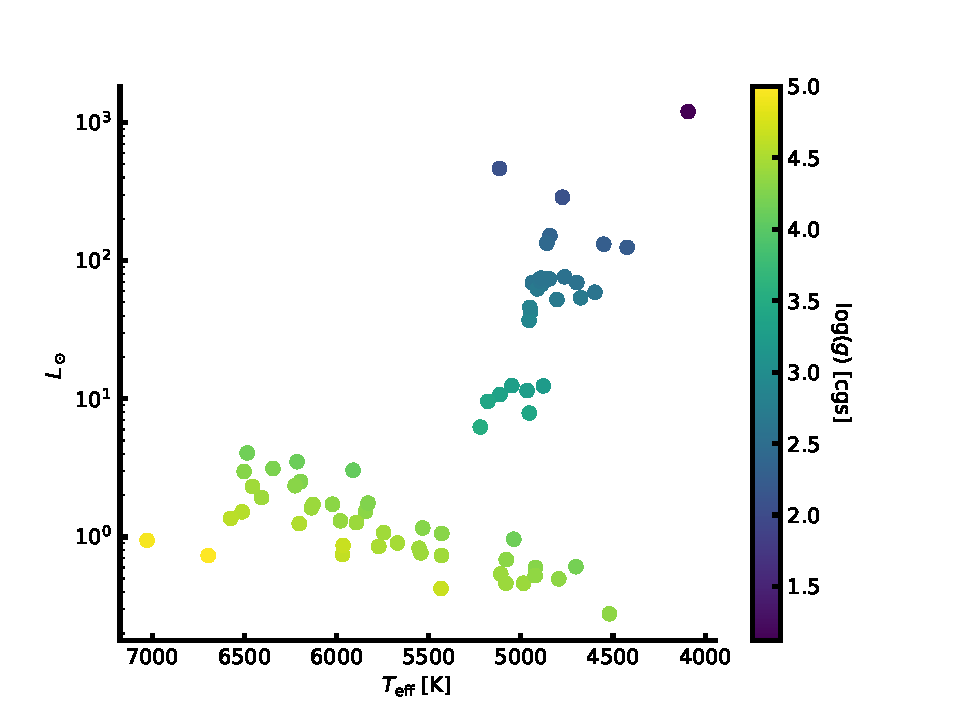
\includegraphics[width=1.0\linewidth]{figures/HR.pdf}
    \caption{A Hertzsprung-Russell diagram of the sample of 50 planet host stars added to SWEET-Cat.
             The parameters were derived using optical high resolution and high S/N spectra in
             tandem with \code{FASMA} and an optical line list. The colour scale shows the derived
             $\log g$ for each star.}
    \label{fig:sweetcat}
\end{figure}

The parameters were derived using \code{FASMA} with the optical line list compiled by
\citet{Sousa2008a} and \citet{Tsantaki2013} for stars where $T_\mathrm{eff}$ was below \SI{5200}{K}.
All the new derived parameters were added to SWEET-Cat, available for the community.

A correction to the spectroscopic surface gravity ($\log g_\mathrm{spec}$) is applied based on
asteroseismology as found by \citet{Mortier2014} given by:
\begin{align}
  \log g_\mathrm{seis} = \log g_\mathrm{spec} - (3.89\pm0.23)\times 10^{-4}\,T_\mathrm{eff}+2.10\pm0.14,
\end{align}
where $\log g_\mathrm{seis}$ is the corrected surface gravity. This correction is only used for FGK
dwarf stars, i.e. between $\SI{4800}{K}\leq T_\mathrm{eff}\leq\SI{6500}{K}$ and $\log
g\geq\SI{4.2}{dex}$. For stars with a $\log g$ lower than this limit the correction will not be
applied, and if the $\log g$ changes to below this limit after the correction, the spectroscopic
$\log g$ will be used again. The correction for $\log g$ depends on both $T_\mathrm{eff}$ and $\log
g$. The correction can be up to \SI{0.5}{dex}, depending on the $T_\mathrm{eff}$.

With these updated parameters the completeness of SWEET-Cat for stars brighter than V magnitude 10
is 85\% (77\% for stars brighter than 12). For fainter stars it is time expensive to acquire spectra
of the quality needed for this method. Moreover, many of the fainter planet host stars have been
observed with the \emph{Kepler} space mission, where most stars are faint.


\subsection{Habitable zone}
\label{sec:HZ}

The habitable zone of a star is at the distance where liquid water may exists. This distance depends
on $T_\mathrm{eff}$ and the luminosity, but also on the planetary atmosphere and its composition.
Using \citet[equation 3 described in][]{Kopparapu2013} to calculate the inner and upper limits of
the habitable zone. The equation is rather simple:
\begin{align}
 d = \sqrt{\frac{L/L_\odot}{S_\mathrm{eff}}} \si{AU},
 S_\mathrm{eff} = S_{\mathrm{eff},\odot} + aT_\ast + bT_\ast^2 + cT_\ast^3 + dT_\ast^4,
\end{align}
where $T_\ast=T_\mathrm-SI{5780}{K}$, and the coefficients can be found in Table 3 in
\citet{Kopparapu2013}, which depends on the specific model of habitable zone used. Here are used the
``Runaway Greenhouse'' for the inner limit and ``Maximum Greenhouse'' for the outer limit of the
habitable zone. The equation above is only valid for main sequence stars FGKM, thus only stars with
$\log g\geq\SI{4.2}{dex}$ have been included.


It was possible to find three planets within this zone; GJ 785 c, HD 37124 c, and KELT-6 c. These
planets does not have known radii, and their minimum masses are
$(0.076,\,0.652,\,3.710)M_\mathrm{Jupiter}$, respectively. Thus, it is fair to assume they are all
gas planets. All three host stars are metal-poor. A correlation between orbital period and host star
metallicity is known \citep[see e.g.][]{Adibekyan2013}, where metal-poor stars have planets with
higher orbital period. It is thus not a surprise that the three planets found in the habitable zone
all orbit a metal-poor star. A quick summary of the system is shown in \tref{tab:hz}.

\begin{table}[htb!]
    \caption{Host star and planetary properties of GJ 785, HD 37124, and KELT-6; all which have an
             exoplanet in the habitable zone.}
    \label{tab:hz}
    \centering
    \begin{tabular}{lrrr}
      \hline\hline
      Parameter            & GJ 785             & HD 37124           & KELT-6             \\
      \hline
      Stellar parameters   &                    &                    &                    \\
      \hline
      $T_\mathrm{eff}$     & \SI{5087(48)}{K}   & \SI{5460(35)}{K}   & \SI{6246(88)}{K}   \\
      $\log g$             & \SI{4.30(10)}{dex} & \SI{4.26(4)}{dex}  & \SI{4.22(9)}{dex}  \\
      $[\ion{Fe}/\ion{H}]$ & \SI{-0.01(3)}{dex} & \SI{-0.42(3)}{dex} & \SI{-0.22(6)}{dex} \\
      Luminosity           & $0.72L_\odot$      & $1.10L_\odot$      & $2.70L_\odot$      \\
      V magnitude          & 6.13               & 7.68               & 10.38              \\
      \hline
      Planetary parameters &                    &                    &                    \\
      \hline
      Planet               & GJ 785 c           & HD 37124 c         & KELT-6 c           \\
      Period               & \SI{525}{days}     & \SI{885}{days}     & \SI{1276}{days}    \\
      Mass                 & $0.076M_J$         & $0.652M_J$         & $3.710M_J$         \\
      Semi-major axis      & \SI{1.18}{AU}      & \SI{1.71}{AU}      & \SI{2.39}{AU}      \\
      Inner HZ limit       & \SI{0.86}{AU}      & \SI{1.04}{AU}      & \SI{1.56}{AU}      \\
      Outer HZ limit       & \SI{1.53}{AU}      & \SI{1.84}{AU}      & \SI{2.70}{AU}      \\
      \hline
    \end{tabular}
\end{table}

In \fref{fig:HZ} the habitable zone of the stars analysed here are shown along with the location of
the planets. The three systems mentioned above are highlighted in the figure.

\begin{figure}[htpb!]
    \centering
    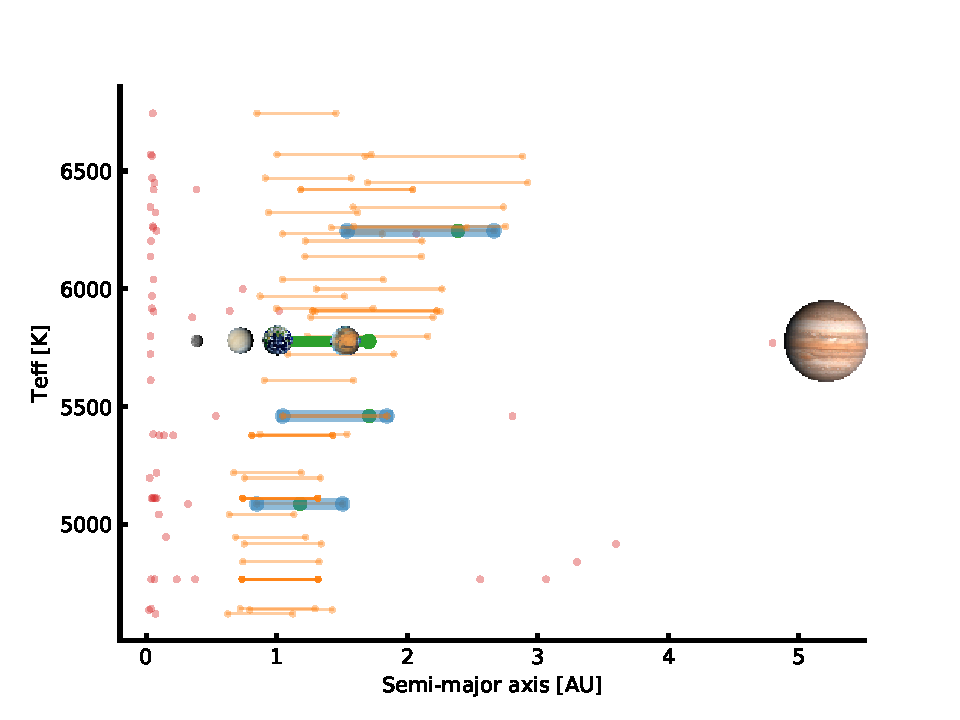
\includegraphics[width=0.8\linewidth]{figures/HZ.pdf}
    \caption{The habitable zone for the updated SWEET-Cat stars. The coloured line shows the
             theoretical habitable zone, while the dots shows the location of the planets in the
             actual system. The blue lines show the habitable zone of the three stars where a planet
             is located within it (green points). The red dots and orange lines are systems which
             does not lie within the habitable zone.}
    \label{fig:HZ}
\end{figure}



\subsection{Changes to planetary parameters}

As a results to the analysis above, it is expected that some planetary parameters will change
compared with the previous literature values.

Therefore the radius and mass of all the 50 new stars updated in SWEET-Cat were computed using the
empirical formula presented in \citet{Torres2010}. Some of the stars have radii derived from
different methods, usually from isochrones. These radii generally show a good correlation with radii
derived from \citet{Torres2010} if the literature parameters of $T_\mathrm{eff}$, $\log g$, and
$[\ion{Fe}/\ion{H}]$ are used. However, when comparing with the new radius derived using the
parameters presented here, the results can differ by up to 65\%. This is shown in \fref{fig:RR} how
the radius calculated from \citet{Torres2010} differs between the literature atmospheric parameters
and the new homogeneous atmospheric parameters presented here. Note that stellar radii are provided
by many of the authors from different discovery papers, but here the atmospheric parameters via the
derivation of the stellar radius, as described above, are compared, rather than comparing the
stellar radii from different methods.

\begin{figure}[tpb]
    \centering
    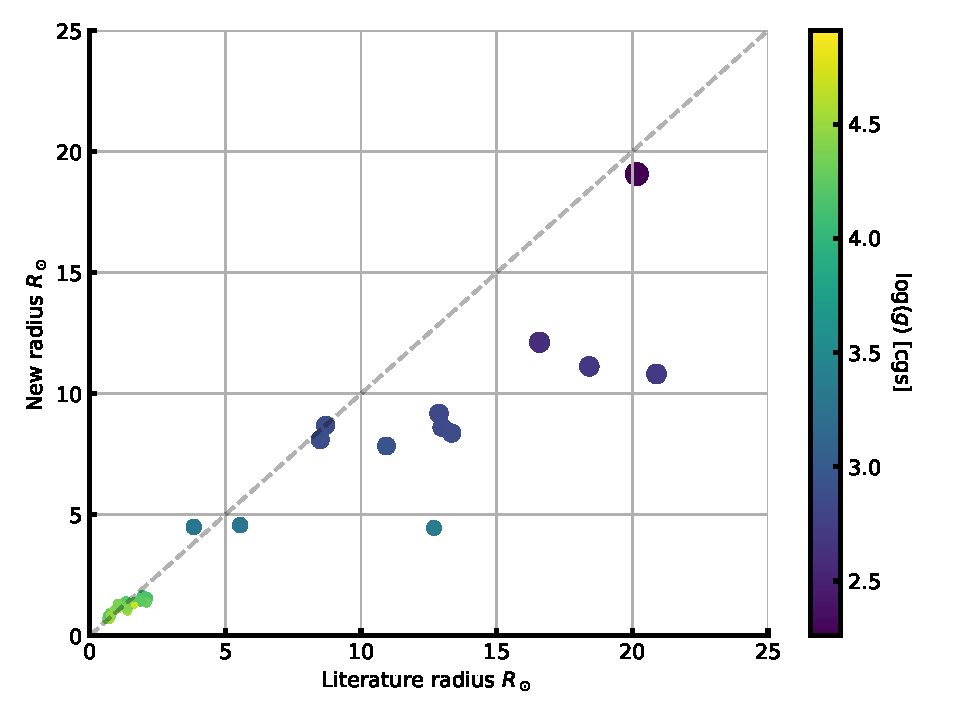
\includegraphics[width=0.8\linewidth]{figures/radiusVSradius.pdf}
    \caption{Stellar radius on both axes calculated based on \citet{Torres2010}. The x-axis shows
             the stellar radius based on the atmospheric parameters from the literature, while the
             y-axis indicates the new homogeneous parameters presented here. The colour and size
             indicate the surface gravity. This clearly shows that the disagreement is biggest for
             more evolved stars.}
    \label{fig:RR}
\end{figure}

In the sections below there follow a discussion of the systems (seven stars, eight exoplanets) where
the radius or mass of the stars changes more than 25\% and how this influences the planetary
parameters. The changes in radius for a star is primarily due to changes in $\log g$, which can be
used as an indicator of the evolutionary stage of a star.

The planetary radius, mass, and semi-major axis were re-derived when possible following the three
simple scaling relations based on Newton's law of gravity \citep{Newton1687} for deriving mass and
distance and simple geometry for radius \citep[see e.g.][]{Torres2008}
\begin{align}
    M_\mathrm{pl,new} &= \left(\frac{M_\mathrm{\ast,lit}}{M_\mathrm{\ast,new}}\right)^{-2/3} M_\mathrm{pl,lit}  \\
    R_\mathrm{pl,new} &= \left(\frac{R_\mathrm{\ast,lit}}{R_\mathrm{\ast,new}}\right) R_\mathrm{pl,lit} \\
    a_\mathrm{pl,new} &= \left(\frac{M_\mathrm{\ast,lit}}{M_\mathrm{\ast,new}}\right)^{1/3} a_\mathrm{pl,lit},
\end{align}
where the subscript ``lit'' denotes the value from the literature used in the comparison, the
subscript ``new'' indicates the new computed values, the subscript ``pl'' is short for planet, and
the subscript ``$\ast$'' is short for star; $M$, $R$, and $a$ are mass, radius, and semi-major axis,
respectively. Note that for the literature values, the values reported directly from the literature
were used and not the derived radius and mass from \citet{Torres2010}. To identify outliers, the
radii and masses were compared when derived from \citet{Torres2010} since this is a measure of how
the atmospheric parameters have changed.


\subsubsection{HAT-P-46}
\label{sub:HAT-P-46}

HAT-P-46 has two known exoplanets according to \citet{Hartmann2014}. The outer planet HAT-P-46 c is
not transiting, hence the radius is not known for this planet. The results presented above for this
star come from UVES/VLT data with a S/N of 208. \citet{Hartmann2014} derived the following
spectroscopic parameters: $T_\mathrm{eff}=\SI{6120(100)}{K}$, $\log g=\SI{4.25(11)}{dex}$, and
$[\ion{Fe}/\ion{H}]=\SI{0.30(10)}{dex}$. Note that for this star the asteroseismic correction
applied (see \sref{sec:sweetcat_analysis}) results in a corrected $\log g$ below 4.2dex, so the
spectroscopic $\log g$ was used for this star.

If mass and radius is derived of HAT-P-46 b with the new parameters, the radius obtained is
$R_\mathrm{pl}=0.93R_J$, while \citet{Hartmann2014} derived $R_\mathrm{pl} = 1.28R_J$. No change in
mass is seen (\citealt{Hartmann2014} found $M_\mathrm{pl}=0.49M_J$); however, there is a decrease in
the radius, and this results with a more dense planet, $\rho_\mathrm{pl}=\SI{0.76}{g/cm^3}$ from
$\rho_\mathrm{pl}=\SI{0.28\pm0.10}{g/cm^3}$.

Only the minimum mass is known for the secondary companions, as it does not transit HAT-P-46 seen
from Earth. With the derived parameters here, the minimum mass is $M\sin i_\mathrm{pl} = 1.97M_J$,
where \citet{Hartmann2014} presented $M\sin i_\mathrm{pl} = 2.00M_J$, so a very small change, as
expected.


\subsubsection{HD 120084}
\label{sub:HD_120084}

The exoplanet orbiting this star with a period of \SI{2082}{days} and a quite eccentric orbit at
0.66 was discovered by \citet{Sato2013}. The atmospheric parameters were derived by
\citet{Takeda2008} using a similar method to that described here. The quality of the spectra they
analysed, however, were not as high as those used here. Using the HIDES spectrograph at the
\SI{188}{cm} reflector at NAOJ, \citet{Takeda2008} reported an average S/N for their sample of
100-300 objects at a resolving power of \num{67000}. The spectrum used here is from ESPaDOnS with a
resolving power of \num{81000}, and with a S/N for this star at 850. With the new parameters
obtained, there is a slight decrease in stellar mass for the star at $1.93M_\odot$ compared to
$2.39M_\odot$ obtained by \citet{Takeda2008}, hence the minimum planetary mass is also slightly
lower, from $m_\mathrm{pl}\sin i=4.5M_J$ to $m_\mathrm{pl}\sin i=3.9M_J$. The stellar radius
decrease by 28\%, from $9.12R_\odot$ to $7.81R_\odot$. Since there are no observations of the planet
transiting, the planetary radius has not been computed.


\subsubsection{HD 233604}
\label{sub:HD_233604}

HD 233604 b was discovered by \citet{Nowak2013}, while the stellar atmospheric parameters of the
star were derived by \citet{Zielinski2012}, who used the same method as described here using the HRS
spectrograph at HET with a resolving power of \num{60000} with a typical S/N at 200-250. For the
analysis presented here, a spectrum from the FIES spectrograph was used with a slightly higher
resolution at \num{67000}, and similar but also slightly higher S/N at 320 for this star.

This planet is in a very close orbit with a semi-major axis of $\sim 15R_\ast$ ($R_\ast$ is the
stellar radius) using the parameters from \citet{Nowak2013}. Using the updated parameters presented
in this paper the stellar mass increase slightly from $1.5M_\odot$ to $1.9M_\odot$, and a decrease
in stellar radius from $10.5R_\odot$ to $8.6R_\odot$. This increases the semi-major axis to $\sim
21R_\ast$. We note that the correct stellar radii are used to describe the semi-major axis in both
cases. The increase in stellar mass leads to an increase in the minimum planetary mass, from
$m_\mathrm{pl}\sin i=6.58M_J$ to $m_\mathrm{pl}\sin i=7.79M_J$.

Moreover, \citet{Nowak2013} found a high \ion{Li}{} abundance at
$A(\ion{Li}{})_\mathrm{LTE}=\SI{1.400\pm0.042}{dex}$ for this star and speculated that this star
might have engulfed a planet. A more likely explanation is that this star has not yet reached the
first dredge-up process \citep{Nowak2013}. In the analysis here a much lower value is found,
$A(\ion{Li}{})_\mathrm{LTE}=\SI{0.92}{dex}$, and hence the star is not believed to be \ion{Li}{}
rich. The \ion{Li}{} abundance found here is in excellent agreement with \citet{Adamow2014}. Even
applying a NLTE correction, as was done in \citet{Adamow2014} ($A(\ion{Li}{})_\mathrm{NLTE}=1.08$),
this star is not \ion{Li}{} rich.


\subsubsection{HD 5583}
\label{sub:HD_5583}

This exoplanet was discovered by \citet{Niedzielski2016} with an orbital period of \SI{139}{days}
around a K giant. This exoplanet was discovered with the radial velocity technique, and the
planetary radius is not known. The stellar parameters were derived in a similar manner to that
presented here \citep[see][and references therein]{Niedzielski2016}; the biggest disagreement is in
the surface gravity. Here was derived a $\log g$ that is higher by \SI{0.34}{dex}, which gives a
stellar radius that is smaller by 37\%. The derived mass is 15\% higher, which in turn increases the
minimum planetary mass from $m_\mathrm{pl}\sin i=5.78M_J$ to $m_\mathrm{pl}\sin i=8.63M_J$. Even
with the increase in mass, it is still within the planetary regime for most inclinations, as was
noted by \citet{Niedzielski2016}.



\subsubsection{HD 81688}
\label{sub:HD81688}

This exoplanet was discovered by \citet{Sato2008} with the RV method. The host star is a metal-poor
K giant. The atmospheric parameters presented in \citet{Sato2008} are obtained via the same method
as presented here, and the agreement is quite good. Once again the big disagreement is in the
surface gravity: Here was obtained \SI{0.48}{dex} higher. Even though the stellar atmospheric
parameters, and hence the planetary parameters, do change, the radius and mass derived are not far
from the values presented in the paper by \citet{Sato2008}. This is a case where the star was marked
as an outlier, due to the comparison between the radius and mass derived from \citet{Torres2010}.

The new stellar mass is the same as before, $2.1M_\odot$. The stellar radius changed from
$13.0R_\odot$ to $10.8R_\odot$. Since a transit of this star has not been observed and the stellar
mass remains the same, there is no change in the planetary parameters.

It is worth noting that this system is in an interesting configuration with a very close orbit
around an evolved star. This system, among others, has been the subject of work on planet engulfment
\citep[see e.g.][]{Kunitomo2011}.


\subsubsection{HIP 107773}
\label{sub:HIP_107773}

The planetary companion was presented in \citet{Jones2015} as an exoplanet around an
intermediate-mass evolved star. The stellar parameters were obtained from the analysis by
\citet{Jones2011} using the same method as presented here, but with a different line list, which
might lead to some disagreements. A higher $\log g$ (\SI{2.83}{dex} compared to \SI{2.60}{dex}) was
derived here, thus the star is slightly smaller with $11.6R_\odot$ to $9.2R_\odot$ and $2.4M_\odot$
to $2.1M_\odot$ for radius and mass of the star, respectively. The other atmospheric parameters are
very similar to those derived by \citet{Jones2011}. This leads to a reduced minimum mass of the
planetary companion from $m\sin i=1.98M_J$ to $m\sin i=1.78M_J$. The planetary radius has not been
measured.



\subsubsection{WASP-97}
\label{sub:WASP-97}

The exoplanet orbiting WASP-97 was discovered by \citet{Hellier2014}. The host star parameters were
derived using a similar method to that described here after co-adding several spectra from the
CORALIE spectrograph. They reach a S/N of 100 with a spectral resolution of \num{50000}. The
parameters presented here come from the UVES spectrograph with a S/N of more than 200.

The parameters do not change much for this planet. The minimum planetary mass changes from
$m_\mathrm{pl}\sin i=1.32M_J$ to $m_\mathrm{pl}\sin i=1.37M_J$ and the radius from $1.13R_J$ to
$1.42R_J$. This affects the density quite strongly; it changes from $\SI{1.13}{g/cm^3}$ to
$\SI{0.59}{g/cm^3}$. This exoplanet is then in the same category as Saturn; its density is lower
than water, but it is slightly larger than Jupiter.

\subsubsection{$\omega$ Serpentis (ome Ser)}
\label{sub:ome_Ser}

The exoplanet orbiting this star with a period of \SI{277}{days} and an eccentric orbit at 0.11 was
also presented by \citet{Sato2013}. The atmospheric parameters were derived in the same way as for
HD 120084. Data from FIES with a resolving power of \num{67000} was used, and with a S/N for this
star of 1168. With the new parameters a slightly higher stellar mass for the star is obtained at
$2.19M_\odot$ compared to the value of $2.17M_\odot$ obtained by \cite{Takeda2008}. This change is
not significant enough to change the minimum planetary mass at $m_\mathrm{pl}\sin i=1.7M_J$. The
stellar radius decreases by more than one solar radius, from $12.3R_\odot$ to $11.1R_\odot$.
However, since there are no observations of transiting exoplanets, any change in planetary radius
cannot be detected.



\subsubsection{o Ursa Major (omi UMa)}
\label{sub:omiUMa}

omi UMa b was discovered by \citet{Sato2012} using the RV method. The stellar parameters are from
\citet{Takeda2008}, as discussed above. The spectrum used for this star is from ESPaDOnS with a S/N
of more than 500 compared to the value of 100-300 reached for the large sample presented in
\citet{Takeda2008}. The luminosity and mass for omi UMa were obtained from theoretical evolutionary
tracks \citep[see][and references therein]{Sato2012}. The radius was then estimated using the
Stefan-Boltzmann relationship, using the measured luminosity and $T_\mathrm{eff}$.

The parameters presented here mainly differ in the surface gravity: here it is \SI{0.72}{dex} higher
at $\log g=3.36$. This leads to a big change in stellar mass and radius from $3.1M_\odot$ to
$1.6M_\odot$ and $14.1R_\odot$ to $4.5R_\odot$, respectively. \citet{Sato2012} have reported that
omi UMa b is the first planet candidate around a star more massive than $3M_\odot$, which is not
supported by the results presented here. With these updated results, the minimum mass of the planet
is now $m\sin i=2.7M_J$, whereas previously it was $m\sin i=4.1M_J$ \citep{Sato2012}. The exoplanet
is not reported to transit, as seen from Earth, so the radius for this exoplanet is not known, which
would have changed a great deal with these new results.




\section{Discovering two giant planet populations}


SWEET-Cat was recently combined with planetary masses to see two distinctive populations for giant
planets by \citet{Santos2017}. This can be seen in the mass histogram in \fref{fig:giantpopulations}
for the full sample of giant planets, with masses higher than 1 Jupiter mass and lower than 20
Jupiter masses, and for a sample constrained by: $\SI{4000}{K}\leq T_\mathrm{eff} \leq\SI{6500}{K}$
in order to have reliably atmospheric parameters from spectroscopic data, orbital periods above
\SI{10}{days} to avoid hot jupiters whose formation and migration process is debated \citep[see
e.g.]{Ngo2016}, orbital periods below 5 years to allow for the sample to be reasonable complete.
Last only stars brighter than 13 magnitude were included to ensure that the planetary masses can
have been derived with reasonable confidence using the radial velocities.

\begin{figure}[htpb!]
    \centering
    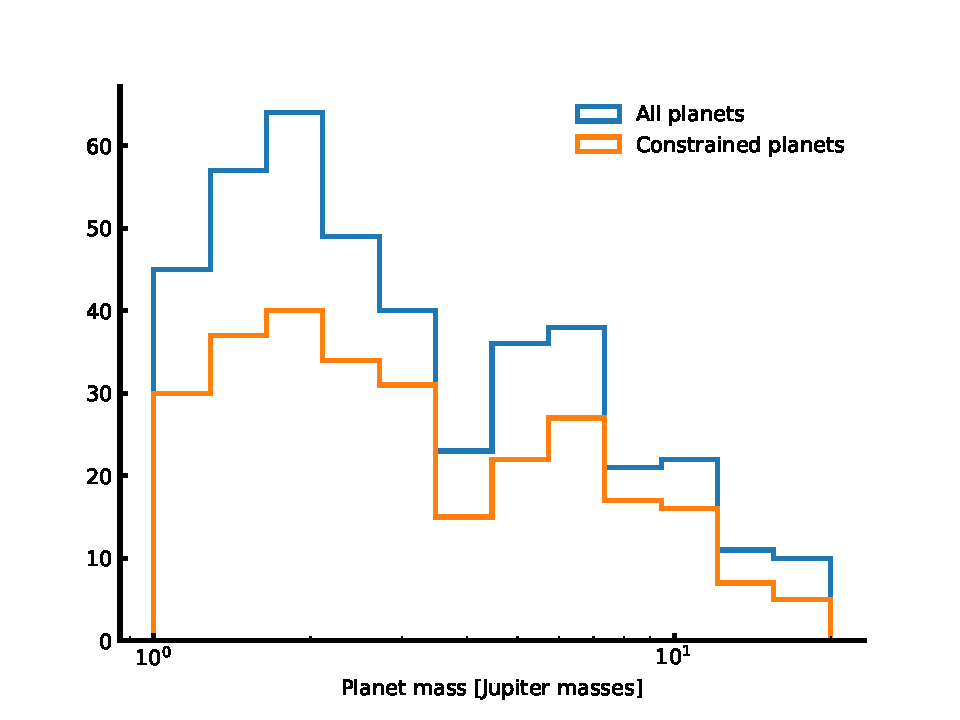
\includegraphics[width=1.0\linewidth]{figures/giantPopulation.pdf}
    \caption{Giant planet masses for the full sample and constrained sample (see text for details).
             This study was performed by \citet{Santos2017} to distinct two giant planet populations.}
    \label{fig:giantpopulations}
\end{figure}

By separating the distribution into two at $4M_{Jup}$, it can be shown \citep[see][for
details]{Santos2017} that the stars hosting the more massive giant planets are in average more
metal-poor compared to the stars hosting the lower mass giant planets. This suggest two different
stellar populations forming giant planets.


\section{Updating SWEET-Cat}

While SWEET-Cat is already a success, it is important to strive to improve the catalogue. Therefore
several improvements for SWEET-Cat are planned. The most important additions are the derivation of
chemical abundances and derivation of mass\footnote{The mass is currently available, however it is
derived from a empirical relation.}, radius, and age using stellar modelling.

With the deviation of chemical abundances, it is possible to make more in-depth studies of the
planet hosts, e.g. by studying trends with condensation temperatures \citep[see
e.g.][]{Adibekyan2016}. By deriving the masses and radii of the planet hosting stars, the planetary
parameters, (mass and radius, and thus the bulk density) can be derived in a consistent way. This
leads to a third improvement of SWEET-Cat; namely re-derived planetary parameters using the
homogeneously derived stellar parameters.

When deriving the stellar masses and radii, the luminosity is also an output, which could be added
to the future version of SWEET-Cat. This leads to simple estimates of the habitable zone limits (see
the discussion above in \sref{sec:HZ}). The implication of this is immediately evident: locating
exoplanets in the habitable zone with the updated stellar parameters. This is of course particular
interesting if the exoplanet is rocky.

Two other additions to SWEET-Cat could be the projected rotational velocity, $v\sin i$, and activity
indicators such as $\log R'_\mathrm{HK}$. Note that $v\sin i$ will be difficult to derive. Here it
is simplest to use synthesis to estimate this parameter, although for slow rotating stars (below
\SI{10}{km/s}) it is difficult to measure accurately with a high precision. These slow rotating
stars are the ones used with the method described above in e.g. \sref{sec:sweetcat_analysis}. The
activity is very important to include, since relations with stellar age and stellar rotation might
be explored. Moreover, some non-obvious correlations such as the correlation found between $\log
R'\mathrm{HK}$ and planetary surface gravity \citep{Hartman2010,Figueira2014} might be explored as
well.

The last update on the wish-list is for the web page itself. It could be made modern with plotting
capabilities, and in tandem combine SWEET-Cat with an exoplanet database, such as
Exoplanet.eu\footnote{\url{http://exoplanet.eu/}}. This will allow any user to quickly explorer
relations between stellar and planetary properties. The tool for plotting has already been developed
and is distributed along with other scripts developed during this PhD under
\code{astro\textunderscore{}scripts}\footnote{Can be found here:
\url{https://github.com/DanielAndreasen/astro_scripts}, and can be installed with \code{pip install
astro-scripts}}.
